\documentclass[draft=false
              ,paper=a4
              ,twoside=false
              ,fontsize=11pt
              ,headsepline
              ,BCOR10mm
              ,DIV11
              ]{scrbook}
\usepackage[ngerman,english]{babel}
%% see http://www.tex.ac.uk/cgi-bin/texfaq2html?label=uselmfonts
\usepackage[ansinew]{inputenc}
%%\usepackage[latin1]{inputenc}
\usepackage{libertine}
\usepackage{pifont}
\usepackage{microtype}
\usepackage{textcomp}
\usepackage[german,refpage]{nomencl}
\usepackage{setspace}
\usepackage{makeidx}
\usepackage{listings}

%%\usepackage{natbib}
\usepackage[backend=biber, style=numeric]{biblatex}
\addbibresource{biblio.bib}

\usepackage[ngerman,colorlinks=true]{hyperref}
\usepackage{soul}
\usepackage{hawstyle}

%% for code snippets
\usepackage{listings}
\usepackage{color}

\definecolor{dkgreen}{rgb}{0,0.6,0}
\definecolor{gray}{rgb}{0.5,0.5,0.5}
\definecolor{mauve}{rgb}{0.58,0,0.82}
%% end code snippet

%% define some colors
\colorlet{BackgroundColor}{gray!20}
\colorlet{KeywordColor}{blue}
\colorlet{CommentColor}{black!60}
%% for tables
\colorlet{HeadColor}{gray!60}
\colorlet{Color1}{blue!10}
\colorlet{Color2}{white}

%% configure colors
\HAWifprinter{
  \colorlet{BackgroundColor}{gray!20}
  \colorlet{KeywordColor}{black}
  \colorlet{CommentColor}{gray}
  % for tables
  \colorlet{HeadColor}{gray!60}
  \colorlet{Color1}{gray!40}
  \colorlet{Color2}{white}
}{}
\lstset{%
  numbers=left,
  numberstyle=\tiny,
  stepnumber=1,
  numbersep=5pt,
  basicstyle=\ttfamily\small,
  keywordstyle=\color{KeywordColor}\bfseries,
  identifierstyle=\color{black},
  commentstyle=\color{CommentColor},
  backgroundcolor=\color{BackgroundColor},
  captionpos=b,
  fontadjust=true
}
\lstset{escapeinside={(*@}{@*)}, % used to enter latex code inside listings
        morekeywords={uint32_t, int32_t}
}
\ifpdfoutput{
  \hypersetup{bookmarksopen=false,bookmarksnumbered,linktocpage}
}{}

%% more fancy C++
\DeclareRobustCommand{\cxx}{C\raisebox{0.25ex}{{\scriptsize +\kern-0.25ex +}}}

\clubpenalty=10000
\widowpenalty=10000
\displaywidowpenalty=10000

% unknown hyphenations
\hyphenation{
}

%% recalculate text area
\typearea[current]{last}

\makeindex
\makenomenclature

\begin{document}
\selectlanguage{ngerman}

%%%%%
%% customize (see readme.pdf for supported values)
\HAWThesisProperties{Author={Marina Knabbe}
                    ,Title={Titel}
                    ,EnglishTitle={English title}
                    ,ThesisType={Bachelorarbeit}
                    ,ExaminationType={Bachelorpr"ufung}
                    ,DegreeProgramme={Bachelor of Science Angewandte Informatik}
                    ,ThesisExperts={Prof. Dr. Erstprüfer \and Prof. Dr. Zweitprüfer}
                    ,ReleaseDate={1. Januar 2345}
                  }

%% title
\frontmatter

%% output title page
\maketitle

\onehalfspacing

%% add abstract pages
%% note: this is one command on multiple lines
\HAWAbstractPage
%% German abstract
{Schlüsselwort 1, Schlüsselwort 2}%
{Dieses Dokument \ldots}
%% English abstract
{keyword 1, keyword 2}%
{This document \ldots}

\newpage
\singlespacing

\tableofcontents
\newpage
%% enable if these lists should be shown on their own page
%%\listoftables
\listoffigures
\lstlistoflistings

\typeout{===== Section: nomenclature}
%% uncomment if a TOC entry is needed
%%\addcontentsline{toc}{chapter}{Glossar}
%%\renewcommand{\nomname}{Glossar}
%%\clearpage
%%\markboth{\nomname}{\nomname} %% see nomencl doc, page 9, section 4.1
%%\printnomenclature

%% main
\mainmatter
\onehalfspacing
%% write to the log/stdout
\typeout{===== File: chapter 1}
%% include chapter file (chapter1.tex)
%%\chapter{Einleitung (unfinished)}
{...
} %% Ende Chapter{Einleitung (unfinished)}

%%%%
%% add some text to generate a sample document
\chapter{Einleitung (unfinished)}
{...
} %% Ende Chapter{Einleitung (unfinished)} %% Einleitung
\chapter{K"unstliche neuronale Netze (unfinished)}
{
\section{Deep Neural Networks / Feedforward Networks (unfinished)}
http://deeplearning4j.org/neuralnet-overview\\
Neural networks are a set of algorithms, modeled loosely after the human brain, that are designed to recognize patterns. They interpret sensory data through a kind of machine perception, labeling or clustering raw input. The patterns they recognize are numerical, contained in vectors, into which all real-world data, be it images, sound, text or time series, must be translated.
They help group unlabeled data according by similarities among the example inputs, and they classify data when they have a labeled dataset to train on. To be more precise, neural networks extract features that are fed to other algorithms for clustering and classification.\\
As you think about one problem deep learning can solve, ask yourself: What categories do I care about? What information can I act upon? Those outcomes are labels that would be applied to data: spam or not\_spam, good\_guy or bad\_guy, angry\_customer or happy\_customer. Then ask: Do I have the data to accompany those labels? Can I find labeled data, or can I create a labeled dataset (with a service like Mechanical Turk or Crowdflower) that I can use to teach an algorithm the correlation between labels and inputs?\\
Deep learning is a name for a certain set of stacked neural networks composed of several layers. The layers are made of nodes. A node is a place where computation happens, loosely patterned on the human neuron, and firing when it encounters sufficient stimuli. It combines input from the data with a set of coefficients, or weights, that either amplify or dampen that input, thereby assigning significance to it in the task the algorithm is trying to learn. These input-weight products are summed and the sum is passed through a node’s so-called activation function, to determine whether and to what extent that signal progresses further in the net to affect the ultimate outcome, say, an act of classification.\\

Here’s a diagram of what one node might look like.
\renewcommand{\figurename}{Abb.}
\begin{figure}[htp]
%%\begin{floatingfigure}[r]{textwidth}
\centering
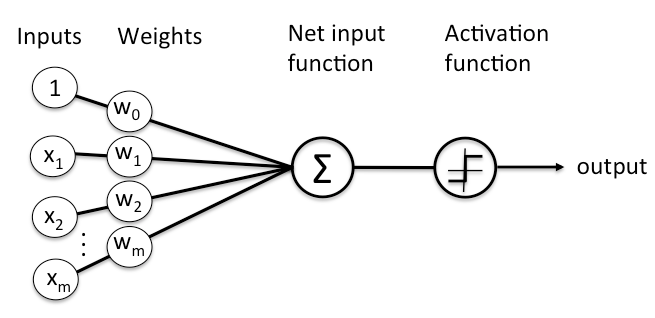
\includegraphics[width=0.75\textwidth]{pictures/perceptron_node.png}
\caption[ein Neuron]{m"ogliches Aussehen eines Neurons\protect\footnotemark}
%%\end{floatingfigure} 
\end{figure}
\footnotetext{Quelle: DL4J \url{http://deeplearning4j.org/neuralnet-overview}}

A node layer is a row of those neuronlike switches that turn on or off as the input is fed through the net. Each layer’s output is simultaneously the subsequent layer’s input, starting from an initial input layer receiving your data.
\renewcommand{\figurename}{Abb.}
\begin{figure}[htp]
%%\begin{floatingfigure}[r]{textwidth}
\centering
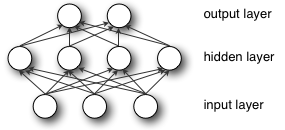
\includegraphics[width=0.50\textwidth]{pictures/mlp.png}
\caption[Aufbau eines neuronalen Netzes]{Aufbau eines neuronalen Netzes\protect\footnotemark}
%%\end{floatingfigure} 
\end{figure}
\footnotetext{Quelle:  DL4J \url{http://deeplearning4j.org/neuralnet-overview}}

Pairing adjustable weights with input features is how we assign significance to those features with regard to how the network classifies and clusters input.

Deep-learning networks are distinguished from the more commonplace single-hidden-layer neural networks by their depth; that is, the number of node layers through which data passes in a multistep process of pattern recognition.

Traditional machine learning relies on shallow nets, composed of one input and one output layer, and at most one hidden layer in between. More than three layers (including input and output) qualifies as "deep" learning. So deep is a strictly defined, technical term that means more than one hidden layer.

In deep-learning networks, each layer of nodes trains on a distinct set of features based on the previous layer’s output. The further you advance into the neural net, the more complex the features your nodes can recognize, since they aggregate and recombine features from the previous layer.

This is known as feature hierarchy, and it is a hierarchy of increasing complexity and abstraction. It makes deep-learning networks capable of handling very large, high-dimensional data sets with billions of parameters that pass through nonlinear functions.

Above all, these nets are capable of discovering latent structures within unlabeled, unstructured data, which is the vast majority of data in the world. Another word for unstructured data is raw media; i.e. pictures, texts, video and audio recordings. Therefore, one of the problems deep learning solves best is in processing and clustering the world’s raw, unlabeled media, discerning similarities and anomalies in data that no human has organized in a relational database or ever put a name to.

For example, deep learning can take a million images, and cluster them according to their similarities: cats in one corner, ice breakers in another, and in a third all the photos of your grandmother. This is the basis of so-called smart photo albums.

Now apply that same idea to other data types: Deep learning might cluster raw text such as emails or news articles. Emails full of angry complaints might cluster in one corner of the vector space, while satisfied customers, or spambot messages, might cluster in others. This is the basis of various messaging filters, and can be used in customer-relationship management (CRM). The same applies to voice messages. With time series, data might cluster around normal/healthy behavior and anomalous/dangerous behavior. If the time series data is being generated by a smart phone, it will provide insight into users’ health and habits; if it is being generated by an autopart, it might be used to prevent catastrophic breakdowns.

Deep-learning networks perform automatic feature extraction without human intervention

Feedforward Networks: Our goal in using a neural net is to arrive at the point of least error as fast as possible. We are running a race, and the race is around a track, so we pass the same points repeatedly in a loop. The starting line for the race is the state in which our weights are initialized, and the finish line is the state of those parameters when they are capable of producing accurate classifications and predictions.

The race itself involves many steps, and each of those steps resembles the steps before and after. Just like a runner, we will engage in a repetitive act over and over to arrive at the finish. Each step for a neural network involves a guess, an error measurement and a slight update in its weights, an incremental adjustment to the coefficients.

Gradient Descent: The name for one commonly used optimization function that adjusts weights according to the error they caused is called "gradient descent."
- describes the relationship between the network’s error and a single weight; i.e. that is, how does the error vary as the weight is adjusted
- for more detailed information visit: http://deeplearning4j.org/neuralnet-overview

Logistic Regression: The mechanism we use to convert continuous signals into binary output is called logistic regression.The name is unfortunate, since logistic regression is used for classification rather than regression in the linear sense that most people are familiar with. It calculates the probability that a set of inputs match the label.
When dealing with labeled input, the output layer classifies each example, applying the most likely label. Each node on the output layer represents one label, and that node turns on or off according to the strength of the signal it receives from the previous layer’s input and parameters.


http://deeplearning4j.org/lstm.html
In the case of feedforward networks, input examples are fed to the network and transformed into an output; with supervised learning, the output would be a label. That is, they map raw data to categories, recognizing patterns that signal, for example, that an input image should be labeled "cat" or "elephant."

\renewcommand{\figurename}{Abb.}
\begin{figure}[htp]
%%\begin{floatingfigure}[r]{textwidth}
\centering
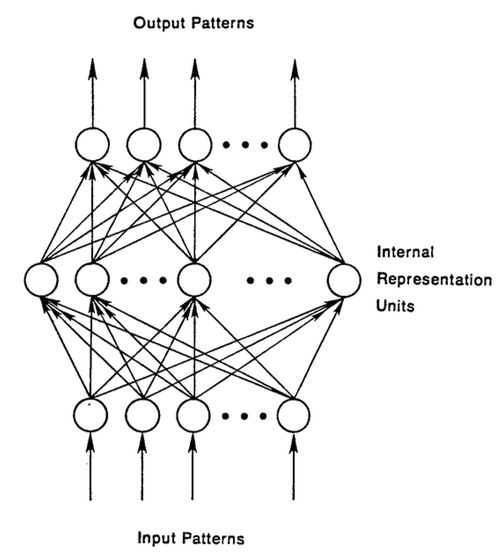
\includegraphics[width=0.60\textwidth]{pictures/feedforward_rumelhart.png}
\caption[Feedforward Netz]{Feedforward Netz\protect\footnotemark}
%%\end{floatingfigure} 
\end{figure}
\footnotetext{Quelle:  DL4J \url{http://deeplearning4j.org/lstm.htm}}

A feedforward network is trained on labeled images until it minimizes the error it makes when guessing their categories. With the trained set of parameters, or weights, the network sallies forth to categorize data is has never seen. A trained feedforward network can be exposed to any random collection of photographs, and the first photograph it is exposed to will not necessarily alter how it classifies the second. Seeing photograph of a cat will not lead the net to perceive an elephant next.

That is, it has no notion of order in time, and the only input it considers is the current example it has been exposed to. Feedforward networks are amnesiacs regarding their recent past; they remember nostalgically only the formative moments of training.


\section{Recurrent Neuronal Networks (RNN) (unfinished)}
http://deeplearning4j.org/lstm.html
Recurrent networks, on the other hand, take as their input not just the current input example they see, but also what they perceived one step back in time.
The decision a recurrent net reached at time step t-1 affects the decision it will reach one moment later at time step t. So recurrent networks have two sources of input, the present and the recent past, which combine to determine how they respond to new data, much as we do in life.
Recurrent networks are distinguished from feedforward networks by that feedback loop, ingesting their own outputs moment after moment as input. It is often said that recurrent networks have memory.2 Adding memory to neural networks has a purpose: There is information in the sequence itself, and recurrent nets use it to perform tasks that feedforward networks can’t.
That sequential information is preserved in the recurrent network’s hidden state, which manages to span many time steps as it cascades forward to affect the processing of each new example.
Given a series of letters, a recurrent will use the first character to help determine its perception of the second character, such that an initial q might lead it to infer that the next letter will be u, while an initial t might lead it to infer that the next letter will be h.

\subsection{Backpropagation Through Time (BPTT)}
Remember, the purpose of recurrent nets is to accurately classify sequential input. We rely on the backpropagation of error and gradient descent to do so.
Backpropagation in feedforward networks moves backward from the final error through the outputs, weights and inputs of each hidden layer, assigning those weights responsibility for a portion of the error by calculating their partial derivatives – ∂E/∂w, or the relationship between their rates of change. Those derivatives are then used by our learning rule, gradient descent, to adjust the weights up or down, whichever direction decreases error.

Recurrent networks rely on an extension of backpropagation called backpropagation through time, or BPTT. Time, in this case, is simply expressed by a well-defined, ordered series of calculations linking one time step to the next, which is all backpropagation needs to work.

Neural networks, whether they are recurrent or not, are simply nested composite functions like f(g(h(x))). Adding a time element only extends the series of functions for which we calculate derivatives with the chain rule.

Truncated BPTT

Truncated BPTT is an approximation of full BPTT that is preferred for long sequences, since full BPTT’s forward/backward cost per parameter update becomes very high over many time steps. The downside is that the gradient can only flow back so far due to that truncation, so the network can’t learn dependencies that are as long as in full BPTT.

\subsection{Vanishing (and Exploding) Gradients}
Like most neural networks, recurrent nets are old. By the early 1990s, the vanishing gradient problem emerged as a major obstacle to recurrent net performance.

Just as a straight line expresses a change in x alongside a change in y, the gradient expresses the change in all weights with regard to the change in error. If we can’t know the gradient, we can’t adjust the weights in a direction that will decrease error, and our network ceases to learn.

Recurrent nets seeking to establish connections between a final output and events many time steps before were hobbled, because it is very difficult to know how much importance to accord to remote inputs. (Like great-great-*-grandparents, they multiply quickly in number and their legacy is often obscure.)

This is partially because the information flowing through neural nets passes through many stages of multiplication.

Everyone who has studied compound interest knows that any quantity multiplied frequently by an amount slightly greater than one can become immeasurably large (indeed, that simple mathematical truth underpins network effects and inevitable social inequalities). But its inverse, multiplying by a quantity less than one, is also true. Gamblers go bankrupt fast when they win just 97 cents on every dollar they put in the slots.

Because the layers and time steps of deep neural networks relate to each other through multiplication, derivatives are susceptible to vanishing or exploding.

Exploding gradients treat every weight as though it were the proverbial butterfly whose flapping wings cause a distant hurricane. Those weights’ gradients become saturated on the high end; i.e. they are presumed to be too powerful. But exploding gradients can be solved relatively easily, because they can be truncated or squashed. Vanishing gradients can become too small for computers to work with or for networks to learn – a harder problem to solve.

Below you see the effects of applying a sigmoid function over and over again. The data is flattened until, for large stretches, it has no detectable slope. This is analogous to a gradient vanishing as it passes through many layers.

\renewcommand{\figurename}{Abb.}
\begin{figure}[htp]
%%\begin{floatingfigure}[r]{textwidth}
\centering
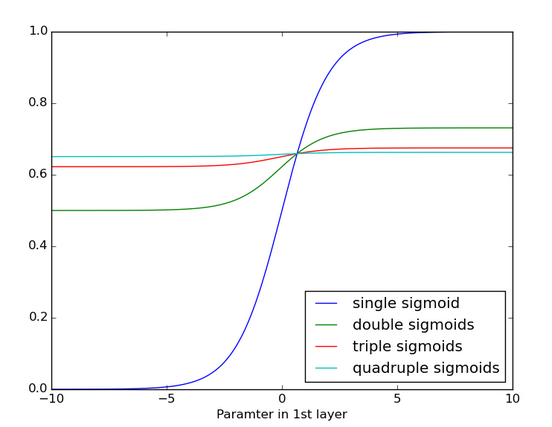
\includegraphics[width=0.60\textwidth]{pictures/sigmoid_vanishing_gradient.png}
\caption[Sigmoid Funktion]{Vanishing Gradient anhand von sigmoid function verdeutlicht\protect\footnotemark}
%%\end{floatingfigure} 
\end{figure}
\footnotetext{Quelle:  DL4J \url{http://deeplearning4j.org/lstm.htm}}


\section{Long Short-Term Memory (LSTM) (unfinished)}
http://deeplearning4j.org/lstm.html
In the mid-90s, a variation of recurrent net with so-called Long Short-Term Memory units, or LSTMs, was proposed by the German researchers Sepp Hochreiter and Juergen Schmidhuber as a solution to the vanishing gradient problem.

LSTMs help preserve the error that can be backpropagated through time and layers. By maintaining a more constant error, they allow recurrent nets to continue to learn over many time steps (over 1000), thereby opening a channel to link causes and effects remotely.

LSTMs contain information outside the normal flow of the recurrent network in a gated cell. Information can be stored in, written to, or read from a cell, much like data in a computer’s memory. The cell makes decisions about what to store, and when to allow reads, writes and erasures, via gates that open and close. Unlike the digital storage on computers, however, these gates are analog, implemented with element-wise multiplication by sigmoids, which are all in the range of 0-1. Analog has the advantage over digital of being differentiable, and therefore suitable for backpropagation.

Those gates act on the signals they receive, and similar to the neural network’s nodes, they block or pass on information based on its strength and import, which they filter with their own sets of weights. Those weights, like the weights that modulate input and hidden states, are adjusted via the recurrent networks learning process. That is, the cells learn when to allow data to enter, leave or be deleted through the iterative process of making guesses, backpropagating error, and adjusting weights via gradient descent.

The diagram below illustrates how data flows through a memory cell and is controlled by its gates.

\renewcommand{\figurename}{Abb.}
\begin{figure}[htp]
%%\begin{floatingfigure}[r]{textwidth}
\centering
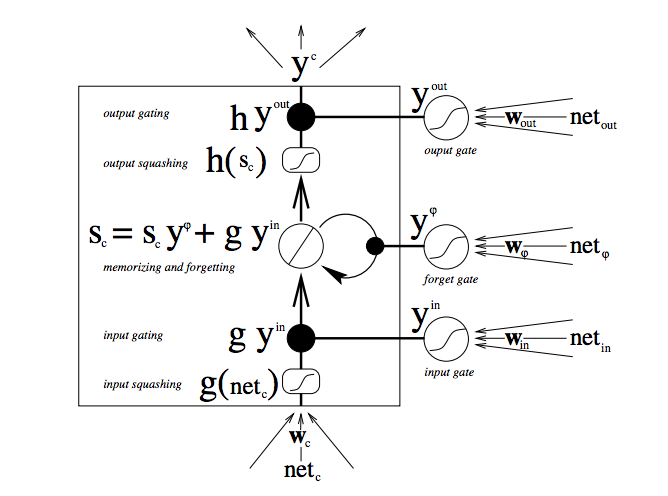
\includegraphics[width=0.60\textwidth]{pictures/gers_lstm.png}
\caption[Memory Cell]{Memory cell\protect\footnotemark}
%%\end{floatingfigure} 
\end{figure}
\footnotetext{Quelle:  DL4J \url{http://deeplearning4j.org/lstm.htm}}

Starting from the bottom, the triple arrows show where information flows into the cell at multiple points. That combination of present input and past cell state is fed not only to the cell itself, but also to each of its three gates, which will decide how the input will be handled.

The black dots are the gates themselves, which determine respectively whether to let new input in, erase the present cell state, and/or let that state impact the network’s output at the present time step. S\_c is the current state of the memory cell, and g\_y\_in is the current input to it. Remember that each gate can be open or shut, and they will recombine their open and shut states at each step. The cell can forget its state, or not; be written to, or not; and be read from, or not, at each time step, and those flows are represented here.

The large bold letters give us the result of each operation.

Here’s another diagram for good measure, comparing a simple recurrent network (left) to an LSTM cell (right). The blue lines can be ignored; the legend is helpful.

\renewcommand{\figurename}{Abb.}
\begin{figure}[htp]
%%\begin{floatingfigure}[r]{textwidth}
\centering
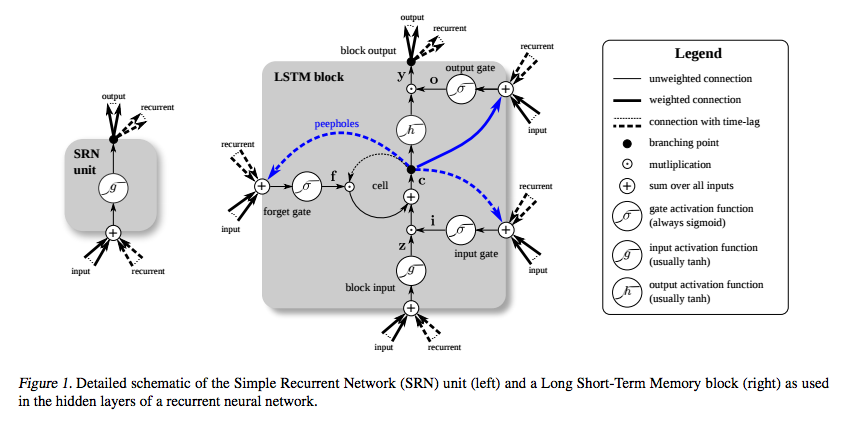
\includegraphics[width=0.60\textwidth]{pictures/greff_lstm_diagram.png}
\caption[Vergleich Recurrent Network und LSTM]{Vergleich: Simple Recurrent Network(SRN) und LSTM block\protect\footnotemark}
%%\end{floatingfigure} 
\end{figure}
\footnotetext{Quelle:  DL4J \url{http://deeplearning4j.org/lstm.htm}}

It’s important to note that LSTMs’ memory cells give different roles to addition and multiplication in the transformation of input. The central plus sign in both diagrams is essentially the secret of LSTMs. Stupidly simple as it may seem, this basic change helps them preserve a constant error when it must be backpropagated at depth. Instead of determining the subsequent cell state by multiplying its current state with new input, they add the two, and that quite literally makes the difference. (The forget gate still relies on multiplication, of course.)

Different sets of weights filter the input for input, output and forgetting. The forget gate is represented as a linear identity function, because if the gate is open, the current state of the memory cell is simply multiplied by one, to propagate forward one more time step.

Furthermore, while we’re on the topic of simple hacks, including a bias of 1 to the forget gate of every LSTM cell is also shown to improve performance.

You may wonder why LSTMs have a forget gate when their purpose is to link distant occurrences to a final output. Well, sometimes it’s good to forget. If you’re analyzing a text corpus and come to the end of a document, for example, you may have no reason to believe that the next document has any relationship to it whatsoever, and therefore the memory cell should be set to zero before the net ingests the first element of the next document.

In the diagram below, you can see the gates at work, with straight lines representing closed gates, and blank circles representing open ones. The lines and circles running horizontal down the hidden layer are the forget gates.

\renewcommand{\figurename}{Abb.}
\begin{figure}[htp]
%%\begin{floatingfigure}[r]{textwidth}
\centering
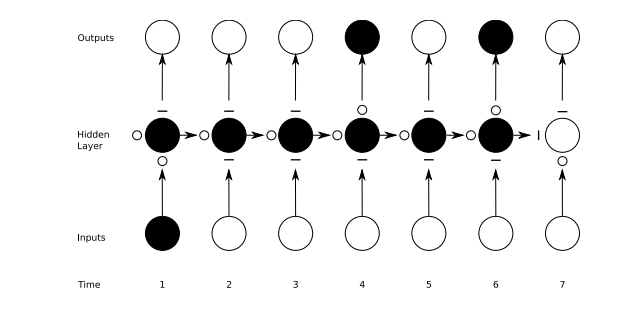
\includegraphics[width=0.60\textwidth]{pictures/gates_lstm.png}
\caption[Gates at work]{Gates at work\protect\footnotemark}
%%\end{floatingfigure} 
\end{figure}
\footnotetext{Quelle:  DL4J \url{http://deeplearning4j.org/lstm.htm}}

It should be noted that while feedforward networks map one input to one output, recurrent nets can map one to many, as above (one image to many words in a caption), many to many (translation), or many to one (classifying a voice).

"Capturing Diverse Time Scales and Remote Dependencies"

You may also wonder what the precise value is of input gates that protect a memory cell from new data coming in, and output gates that prevent it from affecting certain outputs of the RNN. You can think of LSTMs as allowing a neural network to operate on different scales of time at once.

Let’s take a human life, and imagine that we are receiving various streams of data about that life in a time series. Geolocation at each time step is pretty important for the next time step, so that scale of time is always open to the latest information.

Perhaps this human is a diligent citizen who votes every couple years. On democratic time, we would want to pay special attention to what they do around elections, before they return to making a living, and away from larger issues. We would not want to let the constant noise of geolocation affect our political analysis.

If this human is also a diligent daughter, then maybe we can construct a familial time that learns patterns in phone calls which take place regularly every Sunday and spike annually around the holidays. Little to do with political cycles or geolocation.

Other data is like that. Music is polyrhythmic. Text contains recurrent themes at varying intervals. Stock markets and economies experience jitters within longer waves. They operate simultaneously on different time scales that LSTMs can capture.

Further links: (could be sources for pictures)
http://people.idsia.ch/~juergen/rnn.html
https://karpathy.github.io/2015/05/21/rnn-effectiveness/
https://www.cs.cmu.edu/~bhiksha/courses/deeplearning/Fall.2015/pdfs/Werbos.backprop.pdf
http://www.cs.toronto.edu/~graves/phd.pdf
http://www.felixgers.de/papers/phd.pdf
http://arxiv.org/pdf/1503.04069.pdf


https://colah.github.io/posts/2015-08-Understanding-LSTMs/
....

\section{Problemstellungen (unfinished)}
Charakterisierungen ...

http://deeplearning4j.org/lstm.html
Recurrent nets are a type of artificial neural network designed to recognize patterns in sequences of data, such as text, genomes, handwriting, the spoken word, or numerical times series data emanating from sensors, stock markets and government agencies.

} %% Ende Chapter{RNN und LSTM} %% KNN
%%\chapter{Deeplearning4j (unfinished)}
{See also \cite{DL4J}\\von http://deeplearning4j.org/quickstart\\
DL4J targets professional Java developers who are familiar with production deployments, IDEs and automated build tools.\\

\section{Vorraussetzungen und Empfehlungen (unfinished)}
von http://deeplearning4j.org/quickstart\\
- Java 1.7 oder höher (nur 64-Bit Version wird unterstützt\\
- Apache Maven (Maven is a dependency management and automated build tool for Java projects.) check https://books.sonatype.com/mvnex-book/reference/public-book.html for how to use\\
- IntelliJ IDEA oder Eclipse (An Integrated Development Environment (IDE) allows you to work with our API and configure neural networks in a few steps. We strongly recommend using IntelliJ, which communicates with Maven to handle dependencies.)\\
- Git

\section{Getting started (unfinished)}
http://deeplearning4j.org/documentation

\subsection{Installation (unfinished)}
http://deeplearning4j.org/gettingstarted
http://nd4j.org/getstarted.html
http://nd4j.org/dependencies.html

\subsection{Ein Netz erstellen und trainieren (unfinished)}
http://deeplearning4j.org/quickstart.html
Everything starts with a MultiLayerConfiguration, which organizes those layers and their hyperparameters.
Hyperparameters are variables that determine how a neural network learns. They include how many times to update the weights of the model, how to initialize those weights, which activation function to attach to the nodes, which optimization algorithm to use, and how fast the model should learn. This is what one configuration would look like:
\begin{lstlisting}
    MultiLayerConfiguration conf = new NeuralNetConfiguration.Builder()
        .iterations(1)
        .weightInit(WeightInit.XAVIER)
        .activation("relu")
        .optimizationAlgo(OptimizationAlgorithm.STOCHASTIC_GRADIENT_DESCENT)
        .learningRate(0.05)
        // ... other hyperparameters
        .backprop(true)
        .build();
\end{lstlisting}
With Deeplearning4j, you add a layer by calling layer on the NeuralNetConfiguration.Builder(), specifying its place in the order of layers (the zero-indexed layer below is the input layer), the number of input and output nodes, nIn and nOut, as well as the type: DenseLayer.
\begin{lstlisting}
        .layer(0, new DenseLayer.Builder().nIn(784).nOut(250)
                .build())
\end{lstlisting}
Once you’ve configured your net, you train the model with model.fit.

Configuring the POM.xml File

To run DL4J in your own projects, we highly recommend using Maven for Java users, or a tool such as SBT for Scala. The basic set of dependencies and their versions are shown below. This includes:

   -  deeplearning4j-core, which contains the neural network implementations
   -  nd4j-native, the CPU version of the ND4J library that powers DL4J
    - canova-api - Canova is our library vectorizing and loading data



http://deeplearning4j.org/gettingstarted.html
Reproducible Results

Neural net weights are initialized randomly, which means the model begins learning from a different position in the weight space each time, which may lead it to different local optima. Users seeking reproducible results will need to use the same random weights, which they must initialize before the model is created. They can reinitialize with the same random weight with this line:

\begin{lstlisting}
   Nd4j.getRandom().setSeed(123);
\end{lstlisting}

\subsection{LSTM code}
A commented example of a Graves LSTM learning how to replicate Shakespearian drama, and implemented with Deeplearning4j
\subsubsection{Hyperparameter Tuning}
http://deeplearning4j.org/lstm.html
Here are a few ideas to keep in mind when manually optimizing hyperparameters for RNNs:
   - Watch out for overfitting, which happens when a neural network essentially "memorizes" the training data. Overfitting means you get great performance on training data, but the network’s model is useless for out-of-sample prediction.
   - Regularization helps: regularization methods include l1, l2, and dropout among others.
    -So have a separate test set on which the network doesn’t train.
   - The larger the network, the more powerful, but it’s also easier to overfit. Don’t want to try to learn a million parameters from 10,000 examples – parameters > examples = trouble.
  -  More data is almost always better, because it helps fight overfitting.
  -  Train over multiple epochs (complete passes through the dataset).
   - Evaluate test set performance at each epoch to know when to stop (early stopping).
  -  The learning rate is the single most important hyperparameter. Tune this using deeplearning4j-ui; see [this graph] (http://cs231n.github.io/neural-networks-3/\#baby)
  -  In general, stacking layers can help.
  -  For LSTMs, use the softsign (not softmax) activation function over tanh (it’s faster and less prone to saturation (~0 gradients)).
  -  Updaters: RMSProp, AdaGrad or momentum (Nesterovs) are usually good choices. AdaGrad also decays the learning rate, which can help sometimes.
   - Finally, remember data normalization, MSE loss function + identity activation function for regression, Xavier weight initialization


} %% Ende Chapter{Deeplearning4j} %% DL4J
%%\lstset{ %
  backgroundcolor=\color{white},   % choose the background color; you must add \usepackage{color} or \usepackage{xcolor}
  basicstyle=\footnotesize,             % the size of the fonts that are used for the code
  breakatwhitespace=false,            % sets if automatic breaks should only happen at whitespace
  breaklines=true,                 	   % sets automatic line breaking
  captionpos=b,                    	   % sets the caption-position to bottom
  commentstyle=\color{dkgreen},   % comment style
  deletekeywords={...},            	   % if you want to delete keywords from the given language
  escapeinside={\%*}{*)},             % if you want to add LaTeX within your code
  extendedchars=true,                    % lets you use non-ASCII characters; for 8-bits encodings only, does not work with UTF-8
  frame=single,	                        % adds a frame around the code
  keepspaces=true,                         % keeps spaces in text, useful for keeping indentation of code (possibly needs columns=flexible)
  keywordstyle=\color{blue},          % keyword style
  otherkeywords={*,...},                % if you want to add more keywords to the set
  numbers=left,                               % where to put the line-numbers; possible values are (none, left, right)
  numbersep=5pt,                           % how far the line-numbers are from the code
  numberstyle=\tiny\color{gray},   % the style that is used for the line-numbers
  rulecolor=\color{black},                % if not set, the frame-color may be changed on line-breaks within not-black text (e.g. comments (green here))
  showspaces=false,                       % show spaces everywhere adding particular underscores; it overrides 'showstringspaces'
  showstringspaces=false,              % underline spaces within strings only
  showtabs=false,                           % show tabs within strings adding particular underscores
  stepnumber=1,                             % the step between two line-numbers. If it's 1, each line will be numbered
  stringstyle=\color{mauve},          % string literal style
  tabsize=2,	                                  % sets default tabsize to 2 spaces
  title=\lstname                               % show the filename of files included with \lstinputlisting; also try caption instead of title
}

\chapter{Musiksequenzen mit Hilfe von DL4J erzeugen (unfinished)}
{ ...
\section{"Idee" (unfinished)}
- LSTM Netz soll mit Beispielmusik im MIDI-Format gef"uttert werden und daraufhin Musiksequenzen erzeugen

\section{Die Eingabe (unfinished)}
\subsection{Was sind MIDI Files? (unfinished)}
- Musikdatei, Informationen als Events

\subsection{MIDI Files lesen (unfinished)}
- einlesen eines MIDI Files
- Vernachl"assigung des MIDI-Takts

\subsection{DataSets erstellen (unfinished)}
- 2 Varianten implementiert
- umwandeln der eingelesenen MIDI-Events
\subsubsection{Variante 1 (unfinished)}
...
\subsubsection{Variante 2 (unfinished)}
...
\subsubsection{Vergleich der Varianten (unfinished)}
...


\section{Das Netz (unfinished)}
%%\section{Netzwerke erstellen}


\section{Die Ausgabe (unfinished)}
\subsection{MIDI Files schreiben (unfinished)}
\subsection{Ergebnisse (unfinished)}
\subsubsection{Variante 1 (unfinished)}
\subsubsection{Variante 2 (unfinished)}

\section{M"ogliche Erweiterungen und Verbesserungen (unfinished)}

} %% Ende Chapter{Musiksequenzen mit Hilfe von DL4J erzeugen} %% Mein Projekt
%%\chapter{Fazit (unfinished)}
{ ...
} %% Ende Chapter{Fazit} %% Fazit

%% appendix if used
\appendix
%%\typeout{===== File: appendix}
%%\lstset{ %
  backgroundcolor=\color{white},   % choose the background color; you must add \usepackage{color} or \usepackage{xcolor}
  basicstyle=\footnotesize,             % the size of the fonts that are used for the code
  breakatwhitespace=false,            % sets if automatic breaks should only happen at whitespace
  breaklines=true,                 	   % sets automatic line breaking
  captionpos=b,                    	   % sets the caption-position to bottom
  commentstyle=\color{dkgreen},   % comment style
  deletekeywords={...},            	   % if you want to delete keywords from the given language
  escapeinside={\%*}{*)},             % if you want to add LaTeX within your code
  extendedchars=true,                    % lets you use non-ASCII characters; for 8-bits encodings only, does not work with UTF-8
  frame=single,	                        % adds a frame around the code
  keepspaces=true,                         % keeps spaces in text, useful for keeping indentation of code (possibly needs columns=flexible)
  keywordstyle=\color{blue},          % keyword style
  otherkeywords={*,...},                % if you want to add more keywords to the set
  numbers=left,                               % where to put the line-numbers; possible values are (none, left, right)
  numbersep=5pt,                           % how far the line-numbers are from the code
  numberstyle=\tiny\color{gray},   % the style that is used for the line-numbers
  rulecolor=\color{black},                % if not set, the frame-color may be changed on line-breaks within not-black text (e.g. comments (green here))
  showspaces=false,                       % show spaces everywhere adding particular underscores; it overrides 'showstringspaces'
  showstringspaces=false,              % underline spaces within strings only
  showtabs=false,                           % show tabs within strings adding particular underscores
  stepnumber=1,                             % the step between two line-numbers. If it's 1, each line will be numbered
  stringstyle=\color{mauve},          % string literal style
  tabsize=2,	                                  % sets default tabsize to 2 spaces
  title=\lstname                               % show the filename of files included with \lstinputlisting; also try caption instead of title
}

\chapter{DL4J-Projekt in IntelliJ aufsetzen}
{
Nach erfolgreicher Installation von IntelliJ und Maven kann ein DL4J-Projekt mithilfe von Maven eingerichtet werden. Hierf"ur w"ahlt man \glqq File\grqq{} $\rightarrow$ \glqq New\grqq{} $\rightarrow$ \glqq Project ...\grqq . 
\renewcommand{\figurename}{Abb.}
\begin{figure}[htp]
%%\begin{floatingfigure}[r]{textwidth}
\centering
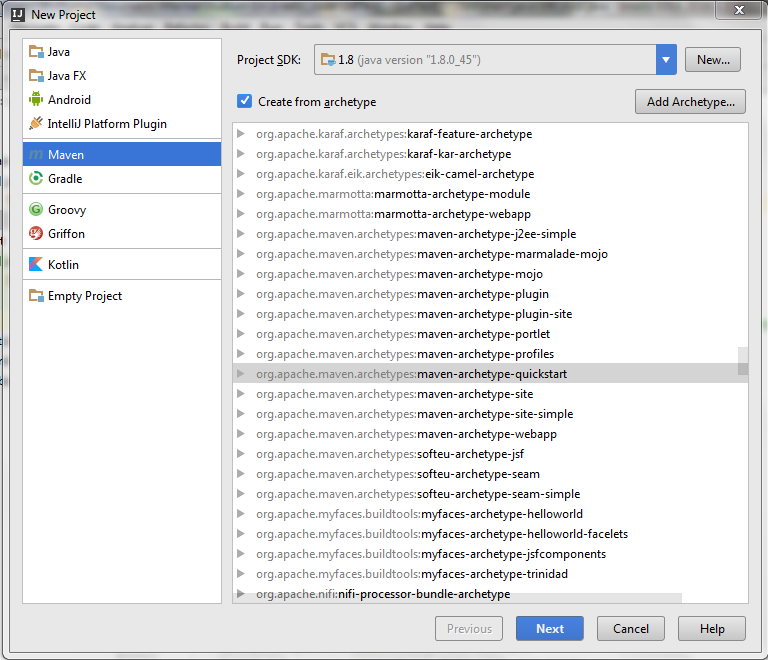
\includegraphics[width=0.80\textwidth]{pictures/mavenProj.png}
\caption[\glqq New Project\grqq{} Fenster]{\glqq New Project\grqq{} Fenster}
%%\end{floatingfigure} 
\end{figure}
Es "offnet sich das \glqq New Project\grqq -Fenster, wie in Abbildung A.1 abgebildet und man w"ahlt auf der linken Seite \glqq Maven\grqq{} (in der Abbildung mit einer roten 1 versehen). Das K"astchen \glqq Create from archetype\grqq{} (in Abbildung gekennzeichnet mit 2) wird ausgew"ahlt und aus der Liste, der verf"ugbaren Typen der Typ \glqq maven-archetype-quickstart\grqq{} (in Abbildung gekennzeichnet mit 3) gew"ahlt. Danach auf \glqq Next\grqq{}  und die GroupId (Package Name) sowie ArtifactId (?) festlegen. Anschlie{\ss}end noch einen Projektname festlegen und \glqq Finish\grqq{} dr"ucken.

http://nd4j.org/getstarted.html

Nachdem Maven f"ur einen die Projektstruktur erstellt hat, muss man die neu erstellte POM.xml Datei noch anpassen. Die POM.xml enth"alt die Projektabh"angigkeiten, welche je Projekt variieren k"onnen. Hier kann man festlegen ob das Projekt auf der CPU oder GPU laufen soll.


The default backend for CPUs is nd4j-native. You can paste that into the $<$dependencies$>$ ... $<$/dependencies$>$ section of your POM like this:
\lstset{language=XML}
\begin{lstlisting}[language=XML,caption=applicationContext.xml]
 <dependency>
   <groupId>org.nd4j</groupId>
   <artifactId>nd4j-native</artifactId>
   <version>${nd4j.version}</version>
 </dependency>
\end{lstlisting}

ND4J’s version is a variable here. It will refer to another line higher in the POM, in the $<$properties$>$ ... 
$<$/properties$>$ section, specifying the nd4j version and appearing similar to this:
\begin{lstlisting}[language=XML,caption=applicationContext.xml]
  <nd4j.version>0.4-rc3.9</nd4j.version>
  <dl4j.version>0.4-rc3.10</dl4j.version>
\end{lstlisting}

The DL4J dependencies you add to the POM will vary with the nature of your project.

In addition to the core dependency, given below, you may also want to install deeplearning4j-cli for the command-line interface, deeplearning4j-scaleout for running parallel on Hadoop or Spark, and others as needed.
\begin{lstlisting}[language=XML,caption=applicationContext.xml]
	   <dependency>
	     <groupId>org.deeplearning4j</groupId>
	     <artifactId>deeplearning4j-core</artifactId>
	     <version>${dl4j.version}</version>
	   </dependency>
\end{lstlisting}

Weitere Informationen bez"uglich GPU Betrieb oder Benutzung andere Betriebssysteme k"onnen auf der \cite{ND4J} Seite nachgeschlagen werden.
}
\addtocontents{toc}{%
  \protect\addtokomafont{chapterentry}{Anhang }
  }
%%\chapter{Maven Projekt}
%%blubbi blub

% bibliography and other stuff
\backmatter

\typeout{===== Section: literature}
%% read the documentation for customizing the style
%%\nocite{*}
%%\printbibliography
\printbibheading[title={Quellenverzeichnis}]
\printbibliography[keyword=other,heading=subbibliography,title={Literatur}]
\printbibliography[keyword=images,heading=subbibliography,title={Bilder}]

%% index
\typeout{===== Section: index}
\printindex

\newpage
\HAWasurency

\end{document}
